\marco{an improvement of this may become part of intro?}

Before Java 8, concrete methods and static methods where not allowed to appear in interfaces.
Java 8 allows static interface methods and introduces
\emph{default methods}, which allow for implementation insides interfaces. This had an important positive consequence that was probably overlooked by the Java design team: the concept of class (in java) is now redundant and unneeded.
We define a subset of Java, called ClassLess Java, where programs and (reusable) libraries can be easily defined and used.
To avoid for some syntactic boilerplate caused by Java not being originally designed to work without classes, we introduce a new annotation:\mixin  provide default
implementations for various methods (e.g. getters, setters, with-methods)
and a mechanism to instantiate objects. \mixin annotation helps programmers to
write less cumbersome code while coding in ClassLess Java;
indeed we think the obtained gain is so high that ClassLess Java with \mixin annotation can be less cumbersome than full Java.


\section{Overview}\label{sec:ep}

\begin{figure}
\centering
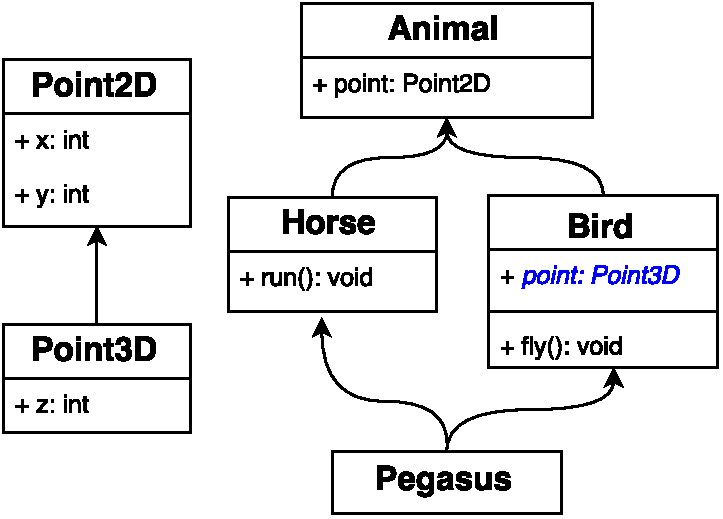
\includegraphics[height=4cm]{PegasusDetail.pdf}
\caption{Pegasus Example.}\label{fig:pegasus}
\end{figure}

\subsection{A Running Example: Animals}
\marco{fig1 is good but is very big, not sure if it worth its space. If we keep it, we need to do it with a vectorial graphic, or better inside latex (for example with tikz)}
To propose a standard example, we show \Q@Animal@s with a two dimensional \Q@Point2D@ representing their \Q@location@.
Some kinds of animals are \Q@Horse@s and \Q@Bird@s.
Birds can \Q@fly@, thus their location need to be a three dimensional \Q@Point3D@.
Finally, we model \Q@Pegasus@ as a kind of \Q@Animal@ with the skills of both \Q@Horse@s and \Q@Bird@s.\footnote{
Some research argues in favour of using subtyping for modelling taxonomies, other research argue against this practice, we do not wish to take sides in this argument, but to provide an engaging example.}

%Suppose we want to model an animal system as shown in Fig~\ref{fig:pegasus}. In
%order to model \texttt{Pegasus}, \emph{multiple inheritance} is clearly needed
%in this example. Therefore, in Java we use interfaces instead of classes. An
%\texttt{Animal} has a \texttt{point} field, indicating the current position of
%the animal. \texttt{Horse} and \texttt{Bird} are subtypes of \texttt{Animal},
%with methods \texttt{run()} and \texttt{fly()}, respectively. Note that
%\texttt{Bird} can fly, therefore refines the type of \texttt{point} from
%\texttt{Point2D} to \texttt{Point3D}. Pegasus (one of the best known creatures
%in Greek mythology) can not only \emph{run} but also \emph{fly}! This is the
%place where \emph{``multiple inheritance''} is needed, because \texttt{Pegasus}
%need to obtain \texttt{fly} and \texttt{run} functionality from both
%\texttt{Horse} and \texttt{Bird}.
%---------------
% We can put more in dept discussion while discussing the classes in details.
%--------------
\subsubsection{\Q@Point2D@: simple immutable data with fields}
Since in ClassLess Java there are no classes, our \Q@Point2D@ must be an interface, as for example:
\begin{lstlisting}
interface Point2D{ int x(); int y();}
\end{lstlisting}
That is, since Java disallows fields inside interfaces,
 we simulate state by abstract methods.
However, how can we create an instance of \Q@Point2D@ without using classes? 
we can just provide an implementation for \Q@x()@ and \Q@y()@ as in
\begin{lstlisting}
new Point2D(){ public int x(){return 4;} public int y(){return 2;}}
\end{lstlisting}
However we are not required to use this cumbersome syntax\footnote{Available in Java from version ...} for every object allocation.
As programmes do, for ease or reuse, we can encapsulate boring long repetitive code in a method. A static factory method in this case is appropriate:
\begin{lstlisting}
interface Point2D{ int x(); int y();
  static Point2D of(int x, int y){return new Point2D(){
    public int x(){return x;} public int y(){return y;}};}
  }
\end{lstlisting}
This obvious constructor code can be automatically generated by our \mixin annotation.

By annotating the interface \Q@Point2D@, the annotation will generate the shown static method \texttt{of}, mimicking the functionality of a simple minded constructor:
By looking the the methods that need implementation it first detects what are the fields, then 
generate an \Q@of@ method with one argument for each of them.

That is, we can just write
\begin{lstlisting}
@Mixin interface Point2D{ int x(); int y();}
\end{lstlisting}

More precisely, a field or factory parameter is generated for every no-args method requiring implementation whose name does not have special meaning\footnote{Formal definition of \mixin behaviour is provided later.}.
An example of code using \Q@Point2D@ is 
\Q@Point2D.of(42,myPoint.y())@
where we return a new point, using \Q@42@ as x-coordinate, and 
taking all the other informations (only \Q@y@ in this case) from another point.
This pattern is very common when programming with immutable data-structures; it is so common that we decided to support it in our code generation as \Q@with-@ methods, that is:
\begin{lstlisting}
@Mixin interface Point2D{ int x(); int y();
  Point2D withX(int val); 
  Point2D withY(int val);}
\end{lstlisting}
is equivalent to 
\begin{lstlisting}
@Mixin interface Point2D{ int x(); int y();
  default Point2D withX(int val){ return Point2D.of(val,this.y());}
  default Point2D withY(int val){ return Point2D.of(this.x(),val);}  }
\end{lstlisting}
Notice how we can provide implementation for methods in an interface, 
and our annotation generate code only if the method \emph{needs} implementation. In this way is trivial for the programmer to personalize the behaviour if they have any special need.

%Firstly, to model \texttt{Point2D} that has x-coordinate and y-coordinate by an
%interface, we immediately run into the problem of expressing the fields
%\texttt{x} and \texttt{y}.
%interfaces. Method \texttt{withX, withY} creates a new instance of
%\texttt{Point2D} with updated field \texttt{x,y}, respectively.

% Firstly, to model \texttt{Animal} by an interface, we immediately run into the
% problem of expressing the field \texttt{point}. Since in Java there is no way to
% define member fields inside interfaces, we propose to simulate fields by
% abstract methods inside interfaces:

%\lstinputlisting[linerange=46-52]{../UseMixinLombok/src/test/TestAnimal.java}% APPLY:linerange=POINT2D

%\paragraph{Instantiation}
%In Java, to implement an interface like \texttt{Point2D}, a typical and trivial
%approach that programmers usually do is creating a class extending the interface
%and providing implementation for all methods inside. For example, this is the
%implementation for interface \texttt{Point2D}:

%\begin{lstlisting}
%class Point2DImpl implements Point2D {
%    private int _x;
%    private int _y;
%    public Point2DImpl(int x, int y) {
%        this._x = x;
%        this._y = y;
%    }
%    public int x() {
%        return _x;
%    }
%    public int y() {
%        return _y;
%    }
% %Your implementation of with is wrong
%    public Point2D withX(int x) {
%        x(x);
%        return this;
%    }
%    public void x(int x) {
%        _x = x;
%    }
%    public void y(int y) {
%        _y = y;
%    }
%    public Point2D withY(int y) {
%        y(y);
%        return this;
%    }
%}
%\end{lstlisting}
%
%\texttt{Point2DImpl} implements \texttt{Point2D} and provides a constructor with
%quite mechanical code. What's worse, the implementation in \texttt{Point2DImpl}
%may not be reused in a single inheritance language.

%
%\begin{lstlisting}
%  // inside interface Point2D
%  static Point of(int x, int y) {
%      return new Point() {
%          int _x = x;
%          int _y = y;
%          public int x() {
%            return _x;
%          }
%          public int y() {
%            return _y;
%          }
%          public Point2D withX(int x) {
%            x(x);
%            return this;
%          }
%          public void x(int x) {
%            _x = x;
%          }
%          public void y(int y) {
%            _y = y;
%          }
%          public Point2D withY(int y) {
%            y(y);
%            return this;
%          }
%    }
%  }
%\end{lstlisting}
%
%\lstinputlisting[linerange=15-27]{../UseMixinLombok/src/overview/TestPoint.java} % APPLY:linerange=POINT_OF

\subsubsection{\Q@Animal@ and \Q@Horse@: simple mutable data with fields}
\Q@Points2D@ are mathematical entities, thus we chosen to use immutable data structure to model them; however animals are real world entities, and when an animal moves, it is the same animal that have now a different location. We model this with mutable state.
%Now we proceed to define \texttt{Animal} with \texttt{point} ``member
%field''.
%%Not again, before we used only getters!
% Again, we model this member field with getter and setter methods:
\lstinputlisting[linerange=64-67]{../UseMixinLombok/src/test/TestAnimal.java}% APPLY:linerange=ANIMAL
\marco{TODO: change point into ``location''}
Here we declare abstract getter and setter for the mutable ``field'' \Q@location@.
As you see, we do not apply the \mixin annotation. This is morally equivalent to an abstract class in full Java; that is we do not provide a convenient way to instantiate it.

\lstinputlisting[linerange=71-76]{../UseMixinLombok/src/test/TestAnimal.java}% APPLY:linerange=HORSE

For \texttt{Horse}, concrete implementation of \texttt{run()} method
need to be defined in a default method, where 
we also show the convenience of \emph{with} methods.
% by method
%\texttt{run()}: method \texttt{withX} returns a new point object with field
%\texttt{x} updated by the argument to \texttt{withX}. Without these
%\texttt{with} methods, operations like \texttt{run()} would be much harder to define.

\subsubsection{\Q@Bird@:  field type refinement}
\Q@Bird@ needs a 3D location, thus first of all we define \Q@Point3D@ and
as follows:
\lstinputlisting[linerange=56-60]{../UseMixinLombok/src/test/TestAnimal.java}% APPLY:linerange=POINT3D

Just to give you a feeling on how much boring code \mixin is generating,  we show the correspondent code without then \mixin annotation\footnote{
As you can see, the generated code is very repetitive, writing such code by hand can easily induce bugs, for example a distract programmer may
swap the arguments of one of the many calls of \Q@Point3D.of@.
}.\begin{lstlisting}
interface Point3D extends Point2D{
  Point3D withX(int val);
  Point3D withY(int val);
  Point3D withZ(int val);
  Point3D with(Point2D val);
  public static Point3D of(int x, int y, int z){return new Point3D(){
    public int x(){return x;} 
    public int y(){return y;}
    public int z(){return z;}
    public Point3D withX(int val){return Point3D.of(val,this.y(),this.z());}
    public Point3D withY(int val){return Point3D.of(this.x(),val,this.z());}
    public Point3D withZ(int val){return Point3D.of(this.x(),this.y(),val);}
    public Point3D with(Point2D val){
      if(val instanceof Point3D){return (Point3D)val;}
      return Point3D.of(val.x(),val.y(),this.z());
      }
    };
  }
}
\end{lstlisting}
Note how \Q@with-@ methods are automatically refined in their return type, so that code like 
\Q@Point3D p=Point3D.of(1,2,3); p=p.withX(42);@ will be accepted and behave as expected. If the programmer wishes to suppress this behaviour and keep the signature as it was, it is sufficient to redefine the \Q@with-@ methods in the new class repeating the old signature.
Again, the philosophy is that if the programmer provides something directly, \mixin do not touch it.
\Q@with-@ methods (functionally) update a field/property at a time.
This can be inefficient, and sometime hard to maintain.
Often we want to update many fields at the same time, for example using another object as source.
Following this idea, the method \Q@with(Point2D)@ is an example of a (functional) properties updater: 
it takes a certain type and in the current object update all field in that type that match fields in the current type.
The idea is that we want as result something that is still like \Q@this@, but modified to be as much as possible similar to the parameter.
The cast in \Q@with(Point2D)@ is trivially safe since it is guarded by an \Q@instanceof@ test. The idea is that if the parameter is a subtype of the current exact type, then we can just return the parameter, as something that is just ``more'' than \Q@this@.

\Q@Bird@s are \Q@Animal@s, 
but while \Q@Animal@s, only need 2D locations,
\Q@Bird@s need  3D locations.
In Java if we define an animal class with a field we have a set of unsatisfactory options in front of us:
\begin{itemize}
\item Define a \Q@Point3D@ field in \Q@Animal@:
this is bad since all animals would require more that is needed, and also it may requires the programmer to predict the future, or it may require to adapt the old code to accommodate for new evolutions.
\item Define a \Q@Point2D@ field in \Q@Animal@ and...
\item Define an extra \Q@int z@ field in \Q@Bird@.
This solution is very at-hoc, requires to basically duplicate the difference between \Q@Point2D@ and \Q@Point3D@ inside of \mbox{\Q@Bird@}.
Again, there are many reasons this would be bad, the most dramatic is that it would not scale to a scenario when the programmer of \Q@Bird@ and the programmer of \Q@Point3D@ are different.
\item Redefine getters and setters in \Q@Bird@, always put \Q@Point3D@ objects in the field and cast
the value out of the \Q@Point2D@ field to \Q@Point3D@ when implementing the overridden getter.
This solution scales to the multiple programmers approach, but requires ugly casts and can be implemented in a wrong way leading to bugs.
\end{itemize}

Many here would think that a language extension is needed.
Instead, with our language \emph{restriction} the problem can be easily challenged\footnote{Often in programming languages ``freedom is slavery''.}:

\lstinputlisting[linerange=80-88]{../UseMixinLombok/src/test/TestAnimal.java}% APPLY:linerange=BIRD

%Interface \texttt{Point3D} extends \texttt{Point2D} with a new abstract method
%\texttt{int z()} (treated as a getter for member field \texttt{z}). Note that
%the return type of various methods (e.g. with- methods, getters) get refined
%either by covariant method overriding or automatically by our annotation
%processor. Besides \emph{with}, other methods (including \emph{clone},
%\emph{of}) also do type-refinements automatically.

Note how
\begin{itemize}
\item by covariant method overriding we refine the type of our field
\item by \emph{overloading} we define a new setter with the more precise type
\item by default method we provide an implementation for the setter called with the old signature.
\end{itemize}

From the type perspective, the key is the covariant method overriding; however from the semantic perspective the key is the implementation for the setter with the old signature:
by using the \Q@with@ method we may use the information for \Q@z@ already stored in the object to forge an appropriate \Q@Point3D@ to store.
Note how all the informations about what fields sits in \Q@Point3D@ and what in \Q@Point2D@ is properly encapsulated in the \Q@with@ method, and is transparent for the implementer of \Q@Bird@.

\subsubsection{\Q@Pegasus@ and multiple Inheritance}
The \emph{``multiple inheritance''} case appears at interface
\texttt{Pegasus}.
Pegasus (one of the best known creatures
in Greek mythology) can not only \emph{run} but also \emph{fly}! 
It would be handy if they could obtain \texttt{fly} and \texttt{run} functionality from both \texttt{Horse} and \texttt{Bird}.

 Using interfaces and \mixin annotation,
this can happen transparently.

\lstinputlisting[linerange=96-97]{../UseMixinLombok/src/test/TestAnimal.java}% APPLY:linerange=PEGASUS

Note how  even the non trivial pattern for field type refinement is transparently composed, and our pegasus have a \Q@Point3D@ \Q@location@.
Note that this works because \Q@Horse@ do not perform any field type refinement , otherwise we may have to choose/create a common subtype in order for pegasus to exists.

\begin{comment}
\subsection{A Running Example: \texttt{Point}}
Suppose we want to create a point component that models the a point in space,
that has x-coordinate and y-coordinate. For example, if we create the
\texttt{Point} interface in Java, it would look like this:

\begin{lstlisting}
interface Point {
    int x();
    int y(); 
}
\end{lstlisting}

\texttt{Point} has two (conceptually) member fields \texttt{x} and \texttt{y},
representing the two coordinates of a point. Methods \texttt{int x()} and
\texttt{int y()} serve as \emph{getter} methods. 
% Methods \texttt{void X(int X)} and \texttt{void Y(int Y)} serve as
% \emph{setter} methods. Method \texttt{Point withX(int X)} updates field
% \texttt{X} and returns \textbf{this}.

\subsection{Naive Implementation}
In Java, to implement an interface like \texttt{Point}, a typical and trivial
approach that programmers usually do is creating a class extending the interface
and providing implementation for all methods inside. For example, this is the
implementation for interface \texttt{Point}:

\lstinputlisting[linerange=33-46]{../UseMixinLombok/src/overview/TestPoint.java} % APPLY:linerange=POINTIMPL

\texttt{PointImpl} implements \texttt{Point} and provides a constructor with
quite mechanical code. What's worse, the implementation in \texttt{PointImpl}
may not be reused in a single inheritance language.

\subsection{Our Approach}
Instead of writing a whole another class to provide the implementation for
\texttt{Point}, we annotate on interface \texttt{Point} directly with \mixin:

\lstinputlisting[linerange=6-10]{../UseMixinLombok/src/overview/TestPoint.java} % APPLY:linerange=POINT

The \mixin annotation will generate a static method \texttt{of} inside
\texttt{Point}. The method \texttt{of} mimic the functionality of constructors,
it takes arguments same as constructors and return objects similar to
constructors. It makes use of Java anonymous classes and achieves the same
implementation as \texttt{PointImpl}. 

With our approach, we provide a Java annotation \mixin to provide default
implementations for various methods and a mechanism to instantiate
objects. \mixin annotation helps programmers to write less cumbersome code and
instantiate interfaces in Java. 

\lstinputlisting[linerange=15-27]{../UseMixinLombok/src/overview/TestPoint.java} % APPLY:linerange=POINT_OF
\end{comment}


\begin{comment}
\subsection{More On \mixin}
Besides the benefit of freeing programmers from writing boilerplate code, our
\mixin annotation can also allow programs to mimic multiple inheritance in a
restricted form easily.

\lstinputlisting[linerange=46-52]{../UseMixinLombok/src/test/TestAnimal.java}% APPLY:linerange=POINT2D

\lstinputlisting[linerange=56-60]{../UseMixinLombok/src/test/TestAnimal.java}% APPLY:linerange=POINT3D

\lstinputlisting[linerange=64-67]{../UseMixinLombok/src/test/TestAnimal.java}% APPLY:linerange=ANIMAL

\lstinputlisting[linerange=71-76]{../UseMixinLombok/src/test/TestAnimal.java}% APPLY:linerange=HORSE

\lstinputlisting[linerange=80-88]{../UseMixinLombok/src/test/TestAnimal.java}% APPLY:linerange=BIRD

\lstinputlisting[linerange=96-97]{../UseMixinLombok/src/test/TestAnimal.java}% APPLY:linerange=PEGASUS

Interface \texttt{Point3D} extends \texttt{Point/Point2D} with a new abstract
method \texttt{int z()} (treated as a getter for member field
\texttt{z}). Interface \texttt{Horse} shows the usage and advantage of
\emph{with} methods by method \texttt{run()}: method \texttt{withX} returns a
new point object with field \texttt{x} updated by the argument to
\texttt{withX}. Without these \texttt{with} methods, operations like
\texttt{run()} would be much harder to define. Note that the return type of
various methods get refined automatically by our annotation processor. Besides
\emph{with}, other methods (including \emph{clone}, \emph{of}) also do
type-refinements automatically.

The \emph{``multiple inheritance''} case appears at interface
\texttt{Pegasus}. Pegasuses can not only \emph{run} but also \emph{fly}!
Interface \texttt{Pegasus} obtains \texttt{fly} and \texttt{run} functionality
through interface \texttt{Horse} and \texttt{Bird}. Using \mixin annotation,
actually these is no code at all programmers have to write. The idea of using
default methods inside interfaces was proposed in ~\cite{}. It enables us to do
multiple inheritance, which otherwise is hard to do in Java-like languages that
do not support multiple inheritance, easily.
\end{comment}
